\documentclass[english]{sobraep}


\title{Visual Question Answering with DeepProbLog}


\author{Jorrit Willaert$^{1}$ \\
	\normalsize $^{1}$Catholic University of Leuven, Leuven -- Belgium \\
	\normalsize e-mail: jorrit.willaert@student.kuleuven.be
}

\begin{document}

\maketitle

\begin{abstract}
	TODO
\end{abstract}

\begin{keywords}
	Neuro Symbolic AI, Visual Question Answering, DeepProbLog, Problog, Convolutional Neural Networks
\end{keywords}

%\let\thefootnote\relax\footnotetext{\hspace*{-5mm}This footnote will be used only by the Editor and Associate Editors.~The edition in this area is not permitted to the authors. This footnote must not be removed while editing the manuscript.}

%\section*{NOMENCLATURE}

%\symbolnomenclature{$P$}{Number of poles.}
%\symbolnomenclature{$V_{qd}$}{Stator voltage \textit{dq} components.}
%\symbolnomenclature{$I_{qd}$}{Stator current \textit{dq} components.}	

%~~~~~~~~~~~~~~~~~~~~~~~~~~~~~~~~~~~~~~~~
%Sections
%~~~~~~~~~~~~~~~~~~~~~~~~~~~~~~~~~~~~~~~~

%Introduction

\section{INTRODUCTION}
The Neuro Symbolic AI community is growing rapidly, indicating that people start to recognize the value of the field. The Neuro Symbolic AI field is interested in building a bridge between the robustness of probabilistic knowledge, with the well-known popularity and proven strengths of deep neural networks. DeepProbLog \cite{deepproblog} offers this ability, by using both the strengths of neural networks (i.e. system 1, typical subconscious tasks such as visual recognition, the processing of languages, \dots), along with the strengths of rule-based probabilistic systems (i.e. system 2, slow, sequential thinking such as the derivation of a proof). 

This paper elaborates on an application that requires both systems to be used, namely Visual Question Answering. System 1 will be required in order to gain an understanding of the image under investigation, with in particular their shapes and colors. System 2, on the other hand, will use this extracted information for deriving certain properties of objects\footnote{For example, finding the shape of the green object, or deriving if it is located on the left hand side of the image.}, or even for capturing the relations\footnote{Here, one could think of deriving if an object is located to the left of another object, or also for finding the number of circles in the image.} between the objects. 

\section{LITERATURE SURVEY}
The application focuses on Visual Question Answering (VQA), for which huge datasets are present, along with very sophisticated methods. The best known dataset for VQA is CLEVR \cite{clevr_dataset}, which contains 100k images with one million questions. An example image is given in Figure \ref{fig:sample_image_clevr}, while example questions are:
\begin{itemize}
    \item Are there an equal number of large things and metal spheres?
    \item What size is the cylinder that is left of the brown metal thing that is left of the big sphere?
    \item How many objects are either small cylinders or metal things?
\end{itemize}

\begin{figure}[H]
    \begin{center}
    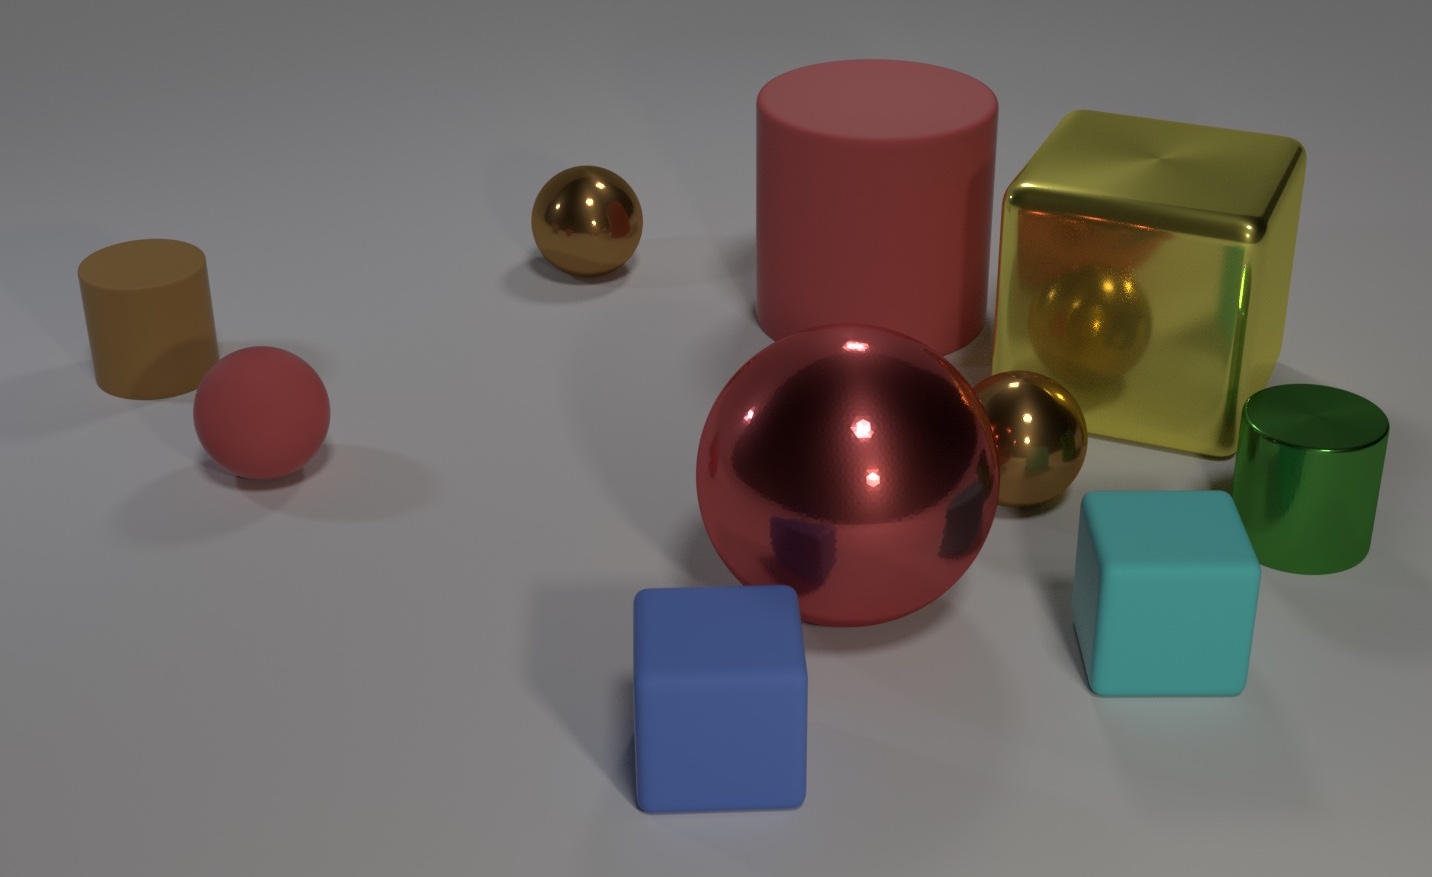
\includegraphics[width=0.3\textwidth]{clevr.jpg}
    \captionsetup{justification=centering}
    \caption{A sample image from the CLEVR dataset \cite{clevr_dataset}}
    \label{fig:sample_image_clevr}
    \end{center}
\end{figure}

Clearly, both system 1 and system 2 are actively used when answering these questions. One could wonder if neural networks alone could answer these questions without having an explicit system 2 encoding (i.e. the rule based knowledge base). Intuitively, it makes sense that if certain facts of the world are known\footnote{They can be encoded, e.g. counting the number of spheres is simply a matter of detecting all the spheres in the image, after which a mathematical summation is a statement in the knowledge base.}, learning can proceed much more quickly\footnote{Not to say that learning might even be impossible if a lot of background knowledge is required.}. Seen from an optimization viewpoint, errors made during prediction in this setup can be targeted exactly, which makes the optimization process also more targeted, and hence more efficient. Finally, this paper also provides evidence for these statements, since in Section \ref{comparison_with_CNN} % TODO ref here
the comparison between this implementation with DeepProbLog is made with a purely CNN based approach. % TODO is this the case?

\section{COMPARISONS WITH PURE SYSTEM 1 APPROACHES}
\label{comparison_with_CNN}

\section{ORGANIZATION OF THE PAPER}
%TODO. Put this above the literature study

This section presents the main issues for editing the manuscript.

\subsection{General Organization}

The papers that shall be published in the Brazilian Power Electronics Journal must contain the following main sections:
1) Title; 2) Authors and Affiliations; 3) Abstract and Keywords; 4) Introduction; 5) Body Text; 6) Conclusions; \linebreak 7) References; 8) Biographies. This order must be respected, unless the authors add some items, such as: Nomenclature; Appendices and Acknowledgements.

Some comments regarding the main items of the manuscripts are presented below.

\subsubsection{Title}

The title of the paper should be as succinct as possible, stating the subject of the paper in a very clear manner. It should be centered at the top of the first page, in bold, type size 14 points, with the whole title in capital letters.

\subsubsection{Authors and affiliations}

Below the title (leaving one blank line), also centered, the name(s) of the author(s) must be included. The middle names may be abbreviated, but the first and last names must be written in their complete forms (type size 12 points). Immediately below the authors' names, their affiliations, with city, state and country, must be informed (type size 10 points).~The electronic addresses must be informed just below the affiliations (type size 10 points).

\subsubsection{Abstract and keywords}

This part is considered one of the most important in the whole paper. It is based on information in Abstract and Keywords that technical papers are indexed and stored in databases.

The Abstract should have no more than 200 words, indicating the main ideas contained in the paper, as well as procedures and obtained results. The Abstract should not be confused with the Introduction and should not have any abbreviations, references, figures, etc. For writing the Abstract, as well as the whole manuscript, you should use passive voice, e. g.,  ``... the experimental results show that...'' instead of ``...~the results we obtained show that...''.~The word Abstract must be written both in italic and in bold. The Abstract text should be in bold.

Keywords are index terms that identify the main topics of the paper. The term Keywords must be both in italic and bold. The Keywords themselves should be in bold.

\subsubsection{Introduction}

The Introduction must prepare the reader for the paper he/she will read, including a historical overview of the subject and also presenting the main contributions of the paper. The Introduction must not be similar to the Abstract and it is the first section of the paper to be numbered as a section.

\subsubsection{Body text}

The authors must organize the body text in various sections, which should contain important information about the proposal of the paper, facilitating its comprehension for readers.

\subsubsection{Conclusions}

The conclusions should be as clear as possible, highlighting the importance of the paper in the respective research area. The advantages and disadvantages of the proposed subject should be clearly emphasized, as well as the obtained results and possible applications.

\subsubsection{References}

The citation of references throughout the text should appear between square brackets, just before the punctuation mark at the end of the sentence in which the reference is inserted. Only the number of the references should be used, avoiding citations such as ``... according to the reference [2]...''.

Papers that were accepted for publication, but were not published yet, should also be in the references along with the citation ``in Press''.

Papers from journals and conferences must begin with the name of the authors (initials followed by the last name), followed by the title, journal or conference name (in italic), number of volume, pages, month and year of publication.

Regarding books, following the name of the authors (initials followed by last name), the title should be in italic, and then should come the publisher, number of edition and place and year of publication.

At the end of these guidelines, there is an example of how the references should be inserted~%\cite{refbib1,refbib2,refbib3,refbib4,refbib5,refbib6,refbib7,refbib8}.

%\nocite{refbib1}
%\nocite{refbib2}
%\nocite{refbib3}
%\nocite{refbib4}
%\nocite{refbib5}
%\nocite{refbib6}
%\nocite{refbib7}
%\nocite{refbib8}



\subsubsection{Biographies}

The biographies of the authors should appear in the same order as in the beginning of the paper and should basically contain the following items:
\begin{itemize}
	\item Full name (in bold and underlined);
	\item Place and year of undergraduation and graduation conclusions;
	\item Professional experience (Institutions and companies in which they have worked, number of patents obtained, areas of expertise, relevant scientific activities, scientific societies in which they are members, etc.). \newline
\end{itemize}

In case additional items are used, such as Nomenclature, Appendices and Acknowledgements, the following instructions should be considered:

\subsubsection{Nomenclature}

The nomenclature consists of the definition of quantities and symbols used throughout the paper. Its inclusion is not mandatory and this item must not be numbered. If this item is included, it should precede the Introduction. In case the authors do not include this item, the  definition of quantities and symbols must occur during the text, right after they appear. In the beginning of these guidelines there is an example of this optional item.

\subsubsection{Acknowledgements and appendices}

The acknowledgements to any collaborators, as well as appendices, do not receive any numeration and should be at the end of the text, before the references. At the end of this text there is an example of this optional item.

On the last page of the paper, the authors should distribute the contents evenly, using both columns, in a way that both end in a parallel manner.

\subsection{Organization of the Sections of the Paper}

The organization of the manuscript in titles and subtitles is important to divide it in sections, which help the reader to find subjects of interest in the paper. They also help the authors to develop their paper in an orderly form. The paper can be organized in primary, secondary and tertiary sections.

The primary sections are the titles of the actual sections. They are written in capital letters in the center of the column separated by a blank line above and another one below them, and sequential Roman numerals should be used.

The secondary sections are the subtitles of the sections. Just the first letter of each word of the section should be written with a capital letter. It should be located at the left part of the column being separated by a blank line above from the rest of the text. The designation of the secondary sections is done with letters in uppercase form, followed by a dot. They should be in italic.

The tertiary sections are subdivisions of the secondary sections. Only the first letter of the first word of the section should be a capital letter. The designation of the tertiary sections should be done with Arabic numerals, followed by parentheses. They should be in italic.

\section{OTHER INSTRUCTIONS}

\subsection{Editorial Rules}

For papers with multiple authors, it is necessary to inform the order of presentation of the authors and filling out the Copyright form at the https://mc04.manuscriptcentral.com/revistaep, authorizing the publication of the paper.

The Brazilian Power Electronics Journal should be considered source of original publication. It reserves its right to make normative, spelling and grammatical modifications in the original files, but respecting the style of the authors. The final versions cannot be sent to the authors.

The published papers will become property of the Brazilian Power Electronics Journal, and its total or partial reprinting must be authorized by SOBRAEP.

Figures, tables and equations should follow the following guidelines.

\subsection{Figures and Tables}

Tables and figures (drawings or pictures) should be inserted in the text right after they are mentioned for the first time, as long as they fit the size of the columns; if necessary, use the whole page. Figures resolution should be at least 300 dpi and vector files should be preferably used for better print quality. Table captions should be above the tables and figure captions should be below the figures. The tables should have titles and they are designated by the word Table, being numbered in sequence by Roman numerals. Table captions must be centered and in bold.

Figures also need captions and they are designated by Figure in the text (Fig. in the caption itself), numbered with Arabic numerals in a sequenced manner, left- and right- justified, as shown in the example. The designation of the parts of a figure is done by adding lowercase letters to the numbers of the figures starting with the letter a, e.g. Figure 1(a).

\begin{figure}[H]
%	\includegraphics[scale=1]{figura.eps}
	\centering
	\caption{Magnetization as a function of applied field. (Note that ``Fig.'' is abbreviated and there is a period after the figure number followed by two spaces.)}
	\label{fig:fig1}
\end{figure}

To better understand graphs, the definition of their axes should be done with words not letters, except when referring to waveforms and phase planes. The units should be between parentheses. For example, use the denomination ``Magnetization (A/m)'', instead of ``M (A/m)''.

Figures and tables should be positioned preferably in the beginning or the end of the column, avoiding putting them in the middle. Avoid tables and figures whose sizes exceed the size of the columns. The figures should preferentially be in black, with a white background, since the printed version of the journal is in black and white. Their lines should be thick, so the impression is readable.

\subsection{Abbreviations and Acronyms}
Abbreviations and acronyms must be defined the first time they are used in the text, e.g. ``... Pulse-Width Modulation (PWM)...''.

\subsection{Equations}
Number equations consecutively with equation numbers in parentheses flush with the right margin, as in (1). The equations should be written in a compact form, centered in the column. If a nomenclature section is not included in the beginning of the text, the quantities should be defined right after the equation, such as:
\begin{equation}
	\Delta I_{L}=I_{o}+\frac{\sqrt{3}}{2}\frac{V_{i}}{Z}
\end{equation}
where:

\symboldescription{$\Delta I_{L}$}{resonant inductor peak current;}
\symboldescription{$I_o$}{load current;}
\symboldescription{$V_i$}{source voltage;}
\symboldescription{$Z$}{characteristic impedance.}

\section{CONCLUSIONS}
This paper was fully written in accordance with the guidelines for submissions of papers in English.


\section*{ACKNOWLEDGEMENTS}
The authors thank John Doe for the collaboration of preparing this paper. This Project was financed by the CNPq (xxyyzz process).


\bibliographystyle{bib_sobraep}
\bibliography{Capita_Selecta_AI_Initial_Idea} 

\balance

\end{document}